% SurakshaNet — B.Tech mid-semester briefing (IIT Ropar)
% Diagram-first Beamer. Compile: tectonic surakshanet_btech.tex
\documentclass[aspectratio=169,11pt,xcolor=table]{beamer}
\usetheme{Madrid}
\usecolortheme{default}
\usepackage{fontspec}
\usepackage{amsmath,amssymb}
\usepackage{booktabs}
\usepackage{array}
\usepackage{tikz}
\usepackage{pgfplots}
\pgfplotsset{compat=1.18}
\usetikzlibrary{
  arrows.meta, positioning, calc, fit, backgrounds,
  shapes.geometric, shapes.misc, shadows, chains, patterns
}

\IfFontExistsTF{Kohinoor Devanagari}{
  \newfontfamily\devafont{Kohinoor Devanagari}
}{
  \newcommand{\devafont}{\sffamily}
}
\newcommand{\hi}[1]{{\devafont #1}}

% Brand
\definecolor{snavy}{HTML}{1B365D}
\definecolor{sorange}{HTML}{E24A1A}
\definecolor{steal}{HTML}{0F7A6C}
\definecolor{sok}{HTML}{1F7A52}
\definecolor{sbad}{HTML}{B42318}
\definecolor{spaper}{HTML}{F4F1EA}
\definecolor{tealsoft}{HTML}{E6F4F1}
\definecolor{navysoft}{HTML}{E8EEF5}
\definecolor{oksoft}{HTML}{E7F5EE}
\definecolor{badsoft}{HTML}{FDECE9}
\definecolor{orangesoft}{HTML}{FDE8E0}

\setbeamercolor{structure}{fg=snavy}
\setbeamercolor{palette primary}{bg=snavy,fg=white}
\setbeamercolor{palette secondary}{bg=steal,fg=white}
\setbeamercolor{palette tertiary}{bg=sorange,fg=white}
\setbeamercolor{title}{fg=snavy}
\setbeamercolor{frametitle}{fg=snavy,bg=spaper}
\setbeamercolor{background canvas}{bg=spaper}
\setbeamercolor{normal text}{fg=snavy}
\setbeamercolor{block title}{bg=snavy,fg=white}
\setbeamercolor{block body}{bg=navysoft,fg=snavy}
\setbeamercolor{block title alerted}{bg=sbad,fg=white}
\setbeamercolor{block body alerted}{bg=badsoft,fg=snavy}
\setbeamercolor{block title example}{bg=steal,fg=white}
\setbeamercolor{block body example}{bg=tealsoft,fg=snavy}
\setbeamercolor{footline}{bg=snavy,fg=white}
\setbeamercolor{author in head/foot}{bg=snavy,fg=white}
\setbeamercolor{title in head/foot}{bg=snavy,fg=white}
\setbeamercolor{date in head/foot}{bg=sorange,fg=white}
\setbeamerfont{frametitle}{series=\bfseries,size=\large}
\setbeamerfont{title}{series=\bfseries,size=\LARGE}
\setbeamertemplate{navigation symbols}{}
\setbeamertemplate{headline}{}
\setbeamertemplate{footline}{}
\setbeamertemplate{page number in head/foot}{}
\setbeamertemplate{itemize item}{\color{sorange}$\blacktriangleright$}
\setbeamersize{text margin left=0.6cm,text margin right=0.6cm}

\title{SurakshaNet}
\author{Aamod Jain \and Pratham Garg}
\institute{Indian Institute of Technology Ropar}
\date{20 September 2026}

% Shared TikZ styles
\tikzset{
  >=Latex,
  font=\small\sffamily,
  card/.style={
    draw=#1, fill=white, line width=0.7pt,
    rounded corners=3pt, align=center, inner sep=5pt,
    text width=2.55cm, minimum height=1.55cm, font=\footnotesize\sffamily
  },
  card/.default=snavy,
  pill/.style={
    rounded corners=6pt, fill=#1, text=white, font=\scriptsize\sffamily\bfseries,
    inner xsep=6pt, inner ysep=2pt
  },
  arr/.style={-{Latex[length=2.1mm]}, line width=1.15pt, draw=sorange},
  flowline/.style={line width=1.5pt, draw=sorange, -{Latex[length=2.4mm]}},
  plane/.style={
    rounded corners=5pt, inner sep=8pt, fill=#1, draw=none
  },
  lab/.style={font=\scriptsize\sffamily\bfseries, text=#1}
}

\newcommand{\term}[2]{%
  {\color{snavy}\textbf{Term --- #1.}} \textit{#2}%
}

\begin{document}

% ------------------------------------------------------------------
\begin{frame}[plain]
\begin{tikzpicture}[overlay,remember picture]
  \fill[snavy] (current page.north west) rectangle ([yshift=-0.92cm]current page.north east);
  \fill[sorange] ([yshift=-0.92cm]current page.north west) rectangle ([yshift=-0.99cm]current page.north east);
  \node[anchor=west,text=white,font=\small\sffamily] at ([xshift=0.55cm,yshift=-0.46cm]current page.north west)
    {\textbf{Indian Institute of Technology Ropar} \textperiodcentered{} B.Tech Project};
  \node[anchor=east,text=white,font=\small\sffamily] at ([xshift=-0.55cm,yshift=-0.46cm]current page.north east)
    {Guide: Geeta Yadav};
  \node[anchor=north west,text=snavy,font=\LARGE\bfseries\sffamily,text width=14.3cm,align=left]
    at ([xshift=0.55cm,yshift=-1.25cm]current page.north west)
    {SurakshaNet: on-device Hinglish abuse detection};
  \node[anchor=north west,text=snavy,font=\large\sffamily,text width=14.3cm,align=left]
    at ([xshift=0.55cm,yshift=-2.12cm]current page.north west)
    {B.Tech mid-semester briefing};
  \node[anchor=north west,text=snavy,font=\small\sffamily]
    at ([xshift=0.55cm,yshift=-2.85cm]current page.north west)
    {Aamod Jain and Pratham Garg \textperiodcentered{} 20 September 2026};
\end{tikzpicture}
\vspace*{3.15cm}
\begin{center}
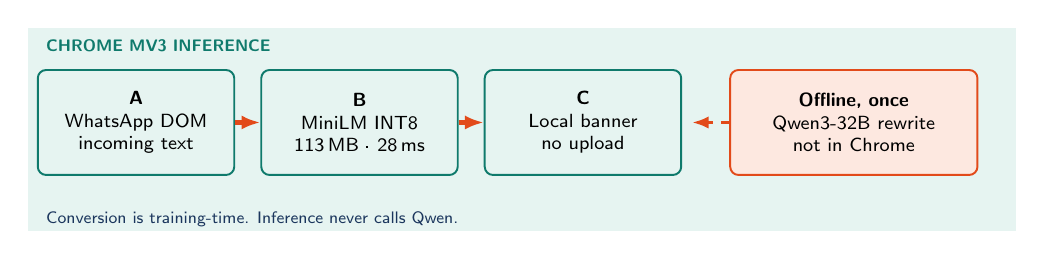
\begin{tikzpicture}[scale=0.86, every node/.style={transform shape}]
  \fill[tealsoft] (0,-1.45) rectangle (14.6,1.55);
  \node[lab=steal,anchor=west] at (0.15,1.28) {CHROME MV3 INFERENCE};
  \node[card=steal,fill=tealsoft] (A) at (1.6,0.15) {\textbf{A}\\WhatsApp DOM\\incoming text};
  \node[card=steal,fill=tealsoft] (B) at (4.9,0.15) {\textbf{B}\\MiniLM INT8\\113\,MB \textperiodcentered{} 28\,ms};
  \node[card=steal,fill=tealsoft] (C) at (8.2,0.15) {\textbf{C}\\Local banner\\no upload};
  \draw[flowline] (A) -- (B);
  \draw[flowline] (B) -- (C);
  \node[card=sorange,fill=orangesoft,text width=3.3cm] (Q) at (12.2,0.15)
    {\textbf{Offline, once}\\Qwen3-32B rewrite\\not in Chrome};
  \draw[arr,dashed] (Q.west) -- ++(-0.55,0);
  \node[font=\scriptsize\sffamily,text=snavy,anchor=west] at (0.15,-1.28)
    {Conversion is training-time. Inference never calls Qwen.};
\end{tikzpicture}
\end{center}
\end{frame}

% ------------------------------------------------------------------
\begin{frame}{Overview}
\begin{center}
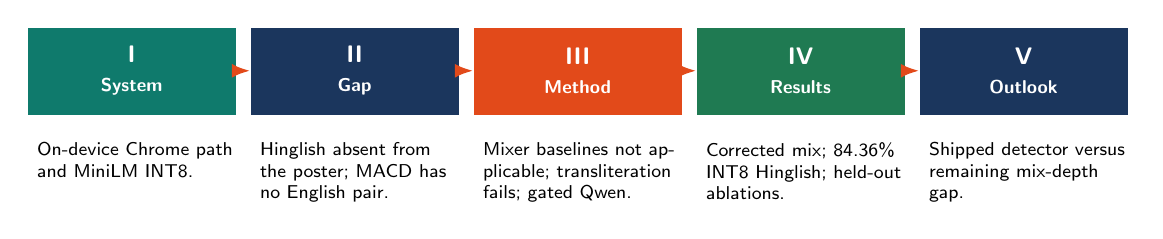
\begin{tikzpicture}[scale=0.96, every node/.style={transform shape}]
  \foreach \x/\lab/\sub/\col in {
    0/I/System/steal,
    2.95/II/Gap/snavy,
    5.90/III/Method/sorange,
    8.85/IV/Results/sok,
    11.80/V/Outlook/snavy} {
    \fill[\col] (\x,0) rectangle (\x+2.75,1.15);
    \node[text=white,font=\bfseries\small\sffamily,align=center] at (\x+1.375,0.58) {\lab\\\scriptsize \sub};
  }
  \draw[flowline] (2.75,0.58) -- (2.95,0.58);
  \draw[flowline] (5.70,0.58) -- (5.90,0.58);
  \draw[flowline] (8.65,0.58) -- (8.85,0.58);
  \draw[flowline] (11.60,0.58) -- (11.80,0.58);

  \node[anchor=north west,text width=2.6cm,font=\scriptsize\sffamily,align=left] at (0,-0.25)
    {On-device Chrome path and MiniLM INT8.};
  \node[anchor=north west,text width=2.6cm,font=\scriptsize\sffamily,align=left] at (2.95,-0.25)
    {Hinglish absent from the poster; MACD has no English pair.};
  \node[anchor=north west,text width=2.6cm,font=\scriptsize\sffamily,align=left] at (5.90,-0.25)
    {Mixer baselines not applicable; transliteration fails; gated Qwen.};
  \node[anchor=north west,text width=2.6cm,font=\scriptsize\sffamily,align=left] at (8.85,-0.25)
    {Corrected mix; 84.36\% INT8 Hinglish; held-out ablations.};
  \node[anchor=north west,text width=2.6cm,font=\scriptsize\sffamily,align=left] at (11.80,-0.25)
    {Shipped detector versus remaining mix-depth gap.};
\end{tikzpicture}
\end{center}
\vspace{0.45em}
{\footnotesize\parbox{\linewidth}{Inference remains the shipped MiniLM path. The Hinglish contribution is a training-set construction that does not alter A--B--C.}}
\end{frame}

% ------------------------------------------------------------------
\begin{frame}{On-device scoring; a cloud round-trip is not a valid design.}
\begin{center}
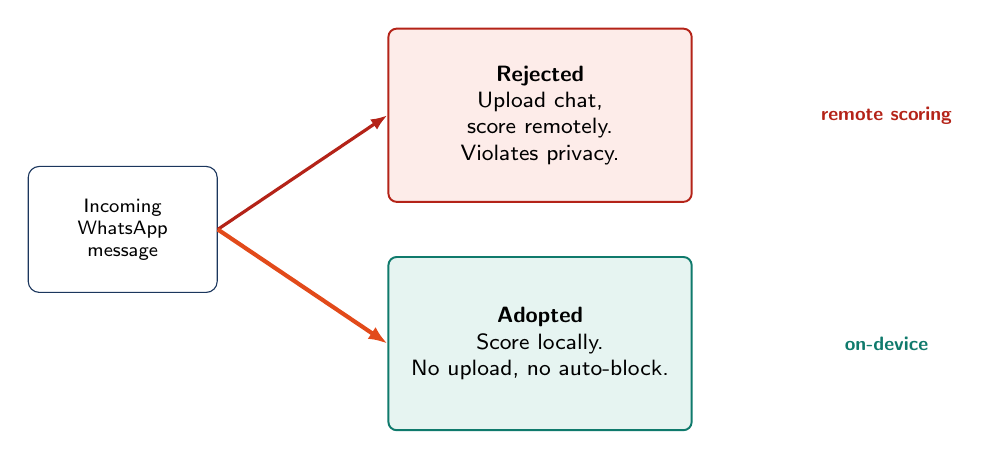
\begin{tikzpicture}
  \node[draw=snavy,rounded corners=4pt,minimum width=2.4cm,minimum height=1.6cm,align=center,font=\scriptsize\sffamily,fill=white] (wa) at (0,0)
    {Incoming\\WhatsApp\\message};
  \node[card=sbad,fill=badsoft,text width=3.5cm,minimum height=2.2cm] (cloud) at (5.3,1.45)
    {\textbf{Rejected}\\Upload chat, score remotely.\\Violates privacy.};
  \node[card=steal,fill=tealsoft,text width=3.5cm,minimum height=2.2cm] (edge) at (5.3,-1.45)
    {\textbf{Adopted}\\Score locally.\\No upload, no auto-block.};
  \draw[arr,sbad] (wa.east) -- (cloud.west);
  \draw[flowline] (wa.east) -- (edge.west);
  \node[font=\scriptsize\sffamily\bfseries,text=sbad] at (9.7,1.45) {remote scoring};
  \node[font=\scriptsize\sffamily\bfseries,text=steal] at (9.7,-1.45) {on-device};
\end{tikzpicture}
\end{center}
\vspace{0.25em}
\term{on-device}{The model, the score, and \texttt{incidents.json} remain on the user's laptop.}
\end{frame}

% ------------------------------------------------------------------
\begin{frame}{Inference path A--B--C; conversion is training-time only.}
\begin{center}
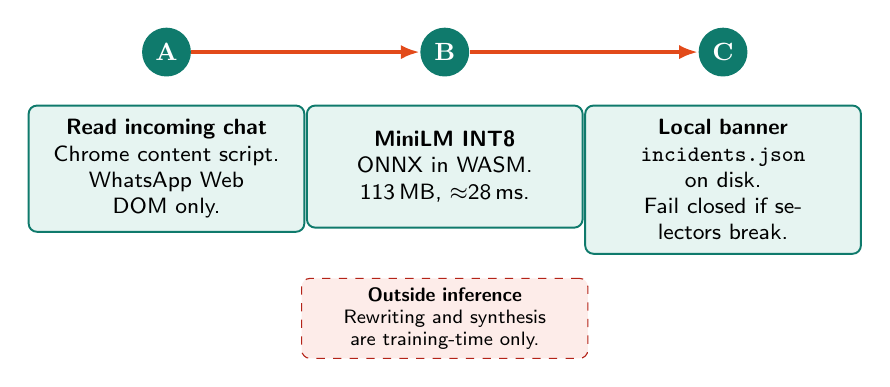
\begin{tikzpicture}[node distance=0.55cm]
  \node[circle,fill=steal,text=white,font=\bfseries\small,minimum size=0.62cm,inner sep=0] (dA) {A};
  \node[circle,fill=steal,text=white,font=\bfseries\small,minimum size=0.62cm,inner sep=0,right=2.9cm of dA] (dB) {B};
  \node[circle,fill=steal,text=white,font=\bfseries\small,minimum size=0.62cm,inner sep=0,right=2.9cm of dB] (dC) {C};
  \draw[flowline] (dA) -- (dB);
  \draw[flowline] (dB) -- (dC);
  \node[card=steal,fill=tealsoft,below=0.35cm of dA,text width=3.15cm] {\textbf{Read incoming chat}\\Chrome content script.\\WhatsApp Web DOM only.};
  \node[card=steal,fill=tealsoft,below=0.35cm of dB,text width=3.15cm] {\textbf{MiniLM INT8}\\ONNX in WASM.\\113\,MB, $\approx$28\,ms.};
  \node[card=steal,fill=tealsoft,below=0.35cm of dC,text width=3.15cm] {\textbf{Local banner}\\\texttt{incidents.json} on disk.\\Fail closed if selectors break.};
  \node[draw=sbad,dashed,rounded corners=3pt,fill=badsoft,text width=3.4cm,align=center,font=\scriptsize\sffamily,below=2.55cm of dB]
    {\textbf{Outside inference}\\Rewriting and synthesis are training-time only.};
\end{tikzpicture}
\end{center}
\vspace{0.15em}
{\footnotesize\term{Chrome MV3}{Current extension platform. Caps bundle size and forbids a silent cloud round-trip at inference.}}
\end{frame}

% ------------------------------------------------------------------
\begin{frame}{XLM-R exceeds the Chrome size budget.}
\begin{center}
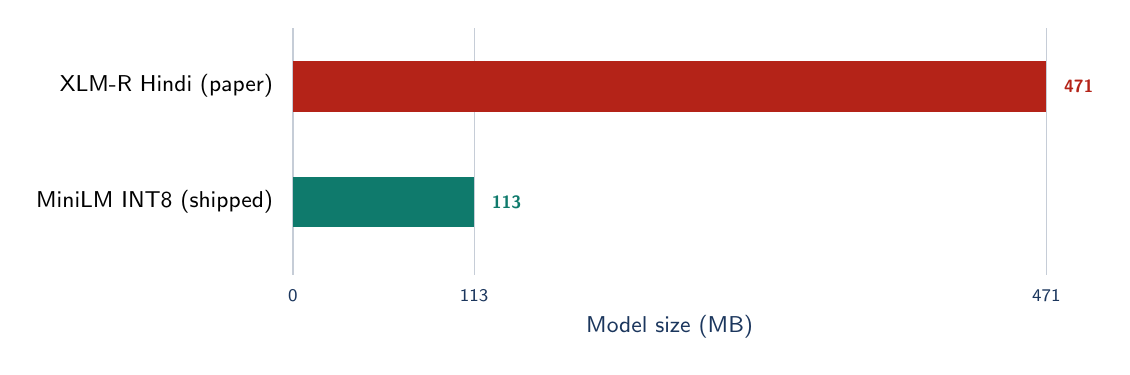
\begin{tikzpicture}[scale=0.92, every node/.style={transform shape}]
  \foreach \x/\lab in {0/0, 2.5/113, 10.4/471} {
    \draw[snavy!25] (\x,0) -- (\x,3.4);
    \node[font=\scriptsize\sffamily,anchor=north,text=snavy] at (\x,-0.08) {\lab};
  }
  \fill[sbad] (0,2.25) rectangle (10.4,2.95);
  \node[font=\small\sffamily,anchor=east] at (-0.15,2.60) {XLM-R Hindi (paper)};
  \node[font=\scriptsize\sffamily\bfseries,text=sbad,anchor=west] at (10.52,2.60) {471};
  \fill[steal] (0,0.65) rectangle (2.5,1.35);
  \node[font=\small\sffamily,anchor=east] at (-0.15,1.00) {MiniLM INT8 (shipped)};
  \node[font=\scriptsize\sffamily\bfseries,text=steal,anchor=west] at (2.62,1.00) {113};
  \node[font=\small\sffamily,text=snavy] at (5.2,-0.72) {Model size (MB)};
\end{tikzpicture}
\end{center}
\vspace{0.15em}
{\footnotesize MACD XLM-R Hindi ceiling is 86.34\%. MiniLM INT8: poster Hindi 84.66\%, drop under 0.11\,pp, 28\,ms.}\\
{\footnotesize\term{INT8}{8-bit quantized ONNX that Chrome loads. FP32 is the training checkpoint.}}
\end{frame}

% ------------------------------------------------------------------
\begin{frame}{Poster evaluation omitted Hinglish.}
\begin{center}
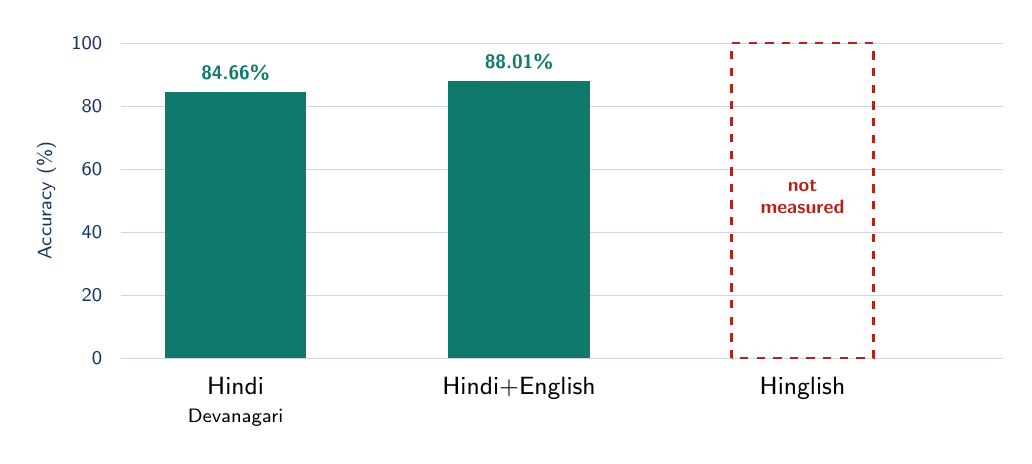
\begin{tikzpicture}
  \foreach \y/\lab in {0/0, 0.8/20, 1.6/40, 2.4/60, 3.2/80, 4.0/100} {
    \draw[snavy!20] (0,\y) -- (11.2,\y);
    \node[font=\scriptsize\sffamily,anchor=east,text=snavy] at (-0.12,\y) {\lab};
  }
  \fill[steal] (0.55,0) rectangle (2.35,3.386);
  \node[font=\scriptsize\sffamily\bfseries,text=steal] at (1.45,3.62) {84.66\%};
  \node[font=\small\sffamily,anchor=north,align=center] at (1.45,-0.12) {Hindi\\[-1pt]{\scriptsize Devanagari}};
  \fill[steal] (4.15,0) rectangle (5.95,3.520);
  \node[font=\scriptsize\sffamily\bfseries,text=steal] at (5.05,3.76) {88.01\%};
  \node[font=\small\sffamily,anchor=north,align=center] at (5.05,-0.12) {Hindi+English};
  \draw[sbad, dashed, line width=0.9pt] (7.75,0) rectangle (9.55,4.0);
  \node[font=\scriptsize\sffamily\bfseries,text=sbad,align=center] at (8.65,2.05) {not\\measured};
  \node[font=\small\sffamily,anchor=north,align=center] at (8.65,-0.12) {Hinglish};
  \node[rotate=90,font=\scriptsize\sffamily,text=snavy] at (-0.95,2.0) {Accuracy (\%)};
\end{tikzpicture}
\end{center}
\vspace{0.15em}
{\footnotesize The dashed bar is a missing measurement, not a score. Subsequent slides fill that cell without changing A--B--C.}
\end{frame}

% ------------------------------------------------------------------
\begin{frame}{Labeled MACD is Devanagari; traffic is Roman Hinglish.}
\begin{center}
\begin{tikzpicture}
  \fill[navysoft] (-0.15,-1.85) rectangle (6.35,2.15);
  \fill[tealsoft] (7.15,-1.85) rectangle (13.65,2.15);
  \node[lab=snavy] at (3.1,1.85) {LABELED CORPUS};
  \node[lab=steal] at (10.4,1.85) {OBSERVED TRAFFIC};
  \node[draw=white,fill=white,rounded corners=3pt,text width=5.5cm,align=left,inner sep=8pt] at (3.1,0.35)
    {\hi{कल मीटिंग है चार बजे}\\[4pt]{\scriptsize Hindi script, Hindi grammar}};
  \node[draw=white,fill=white,rounded corners=3pt,text width=5.5cm,align=left,inner sep=8pt] at (10.4,0.55)
    {\texttt{kal meeting hai 4 baje}\\[3pt]\texttt{bro notes share kar dena}};
  \node[font=\scriptsize\sffamily,text=snavy] at (3.1,-1.45) {Gold labels exist for this script.};
  \node[font=\scriptsize\sffamily,text=steal] at (10.4,-1.45) {This is the register the extension observes.};
  \draw[flowline] (6.35,0.2) -- (7.15,0.2);
\end{tikzpicture}
\end{center}
\term{Hinglish}{Hindi as the matrix language, written in Roman letters, with English words mixed in. Not ITRANS, and not Devanagari in another font.}
\end{frame}

% ------------------------------------------------------------------
\begin{frame}{Training uses published MACD and Davidson labels.}
\begin{center}
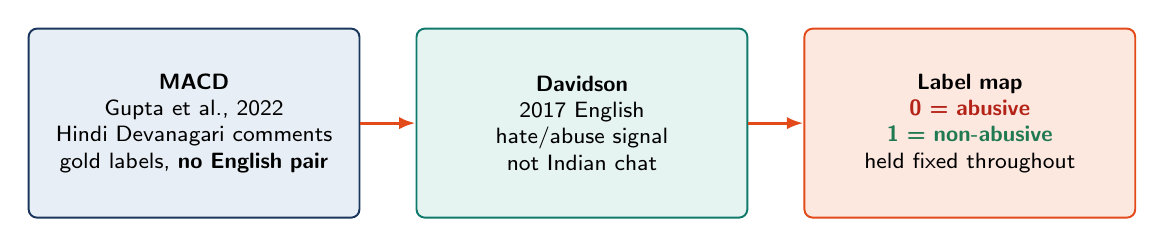
\begin{tikzpicture}[node distance=0.55cm]
  \node[card=snavy,fill=navysoft,text width=3.85cm,minimum height=2.4cm] (m)
    {\textbf{MACD}\\Gupta et al., 2022\\Hindi Devanagari comments\\gold labels, \textbf{no English pair}};
  \node[card=steal,fill=tealsoft,text width=3.85cm,minimum height=2.4cm,right=0.7cm of m] (d)
    {\textbf{Davidson}\\2017 English\\hate/abuse signal\\not Indian chat};
  \node[card=sorange,fill=orangesoft,text width=3.85cm,minimum height=2.4cm,right=0.7cm of d] (l)
    {\textbf{Label map}\\{\color{sbad}\textbf{0 = abusive}}\\{\color{sok}\textbf{1 = non-abusive}}\\held fixed throughout};
  \draw[arr] (m) -- (d);
  \draw[arr] (d) -- (l);
\end{tikzpicture}
\end{center}
\vspace{0.4em}
{\footnotesize\parbox{\linewidth}{\term{MACD}{Multilingual Abusive Comment Detection. ShareChat-scale Hindi comments with published labels.}}}
\end{frame}

% ------------------------------------------------------------------
\begin{frame}{Research question}
\begin{center}

\begin{tikzpicture}
  \fill[white] (0,0) rectangle (13.8,2.15);
  \fill[sorange] (0,2.08) rectangle (13.8,2.15);
  \node[anchor=north west,font=\large\sffamily\bfseries,text=snavy,text width=13.3cm,align=left]
    at (0.25,1.95)
    {Can MACD Hindi be rewritten as conversational Hinglish\\
     with published labels preserved, then measured on a\\
     test frozen before training?};
\end{tikzpicture}
\end{center}
\vspace{0.55cm}
\begin{center}
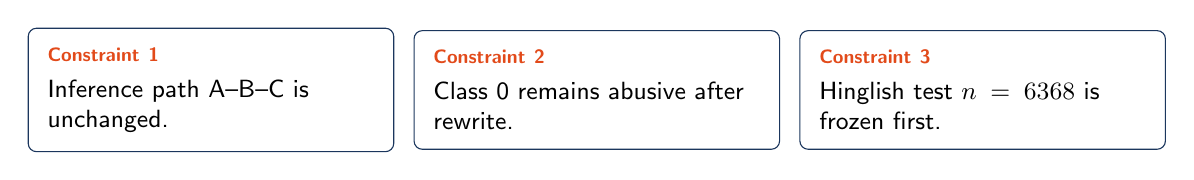
\begin{tikzpicture}
  \foreach \x/\t/\s in {
    0.1/{Constraint 1}/{Inference path A--B--C is \mbox{unchanged}.},
    5.0/{Constraint 2}/{Class 0 remains abusive after rewrite.},
    9.9/{Constraint 3}/{Hinglish test $n=6368$ is frozen first.}} {
    \node[draw=snavy, fill=white, rounded corners=3pt, text width=4.15cm, align=left, inner sep=7pt]
      at (\x+2.15,0) {{\color{sorange}\scriptsize\bfseries \t}\\[2pt]\raggedright\s};
  }
\end{tikzpicture}
\end{center}
\end{frame}

% ------------------------------------------------------------------
\begin{frame}{WAC and PAC require bitext; MACD provides Hindi only.}
\begin{center}
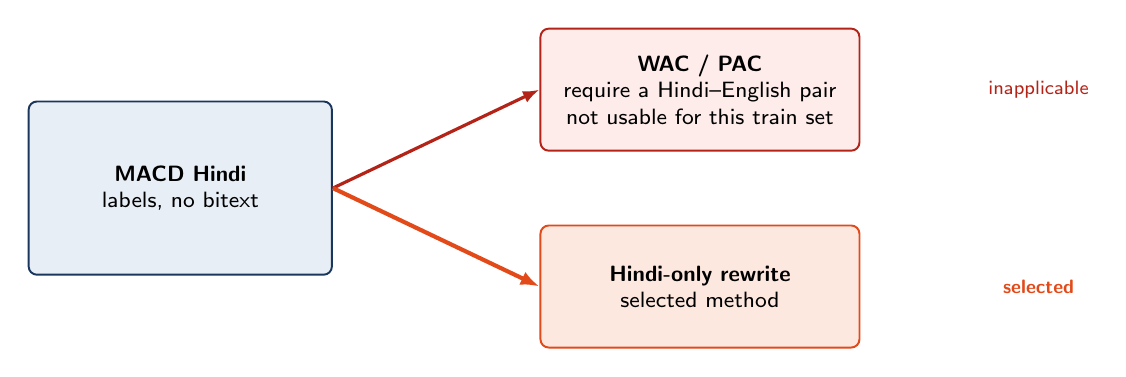
\begin{tikzpicture}
  \node[card=snavy,fill=navysoft,text width=3.5cm,minimum height=2.2cm] (src)
    {\textbf{MACD Hindi}\\labels, no bitext};
  \node[card=sbad,fill=badsoft,text width=3.7cm,minimum height=1.55cm] (wac) at (6.6,1.25)
    {\textbf{WAC / PAC}\\require a Hindi--English pair\\not usable for this train set};
  \node[card=sorange,fill=orangesoft,text width=3.7cm,minimum height=1.55cm] (qw) at (6.6,-1.25)
    {\textbf{Hindi-only rewrite}\\selected method};
  \draw[arr,sbad] (src.east) -- (wac.west);
  \draw[flowline] (src.east) -- (qw.west);
  \node[font=\scriptsize\sffamily,text=sbad] at (10.9,1.25) {inapplicable};
  \node[font=\scriptsize\sffamily\bfseries,text=sorange] at (10.9,-1.25) {selected};
\end{tikzpicture}
\end{center}
\vspace{0.3em}
{\footnotesize\parbox{\linewidth}{\term{HinGE / WAC / PAC}{HinGE: human Hinglish benchmark, $n\approx 1964$ (IITGN). WAC: word-aligned mixing. PAC: phrase-aligned mixing. Both require bitext. HinGE is used later as converter evaluation, not as a train-set builder.}}}
\end{frame}

% ------------------------------------------------------------------
\begin{frame}{Script transliteration is not code-mixing.}
\begin{center}
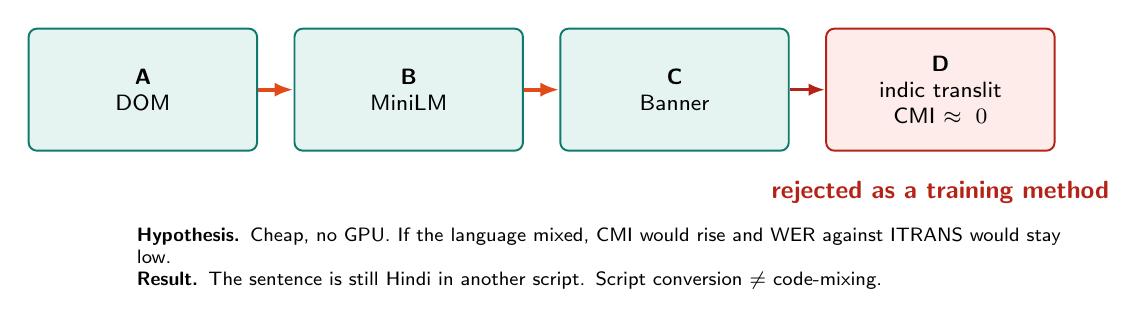
\begin{tikzpicture}
  \node[card=steal,fill=tealsoft] (A) {\textbf{A}\\DOM};
  \node[card=steal,fill=tealsoft,right=0.45cm of A] (B) {\textbf{B}\\MiniLM};
  \node[card=steal,fill=tealsoft,right=0.45cm of B] (C) {\textbf{C}\\Banner};
  \node[card=sbad,fill=badsoft,right=0.45cm of C] (D) {\textbf{D}\\indic translit\\CMI $\approx 0$};
  \draw[flowline] (A) -- (B);
  \draw[flowline] (B) -- (C);
  \draw[arr,sbad] (C) -- (D);
  \node[font=\small\sffamily\bfseries,text=sbad,below=0.25cm of D] {rejected as a training method};
  \node[anchor=west,text width=12cm,font=\scriptsize\sffamily] at (-0.2,-2.15)
    {\textbf{Hypothesis.} Cheap, no GPU. If the language mixed, CMI would rise and WER against ITRANS would stay low.\\
     \textbf{Result.} The sentence is still Hindi in another script. Script conversion $\neq$ code-mixing.};
\end{tikzpicture}
\end{center}
\vspace{0.2em}
\term{CMI}{Code-mixing index (Das \& Gamb\"ack). $0$ = one language. Higher = deeper mix.}\\
\term{WER}{Word error rate $(S+D+I)/N$. Low WER vs ITRANS means ``just transliteration.''}
\end{frame}

% ------------------------------------------------------------------
\begin{frame}{Only conversational Hinglish matches the target register.}
\begin{center}
\begin{tikzpicture}
  \node[card=snavy,fill=white,text width=4.15cm,minimum height=3.3cm] at (0,0)
    {\textbf{1. MACD Hindi}\\[6pt]\hi{कल मीटिंग है चार बजे}\\[8pt]{\scriptsize Labeled corpus. \mbox{Devanagari}. Gold class.}};
  \node[card=sbad,fill=badsoft,text width=4.15cm,minimum height=3.3cm] at (5.0,0)
    {\textbf{2. indic\_transliteration}\\[6pt]\texttt{\small kala mITiMga}\\[-1pt]\texttt{\small hai cAra baje}\\[8pt]{\scriptsize Rejected. Same Hindi. CMI $\approx 0$.}};
  \node[card=sok,fill=oksoft,text width=4.15cm,minimum height=3.3cm] at (10.0,0)
    {\textbf{3. Conversational mix}\\[6pt]\texttt{\small kal meeting hai}\\[-1pt]\texttt{\small 4 baje}\\[8pt]{\scriptsize Target. English words, Hindi grammar.}};
\end{tikzpicture}
\end{center}
\end{frame}

% ------------------------------------------------------------------
\begin{frame}{Qwen3-32B rewrite is offline; it is not in Chrome inference.}
\begin{center}
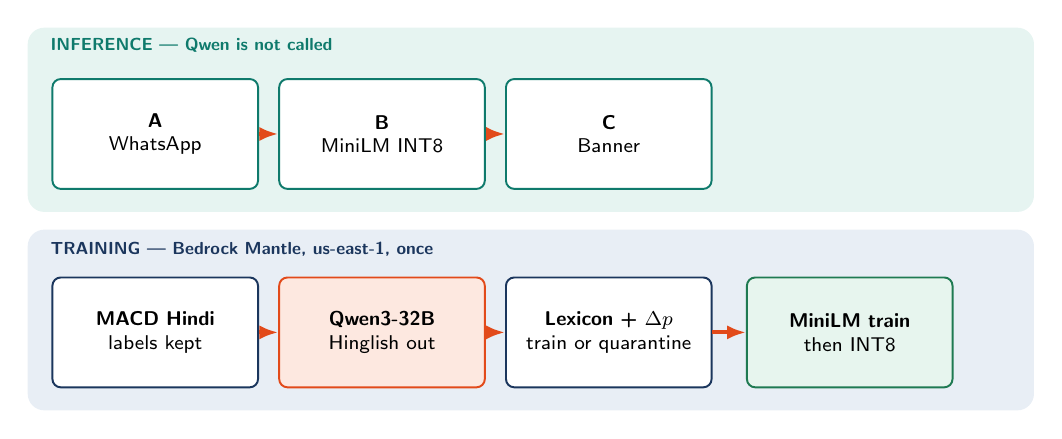
\begin{tikzpicture}[scale=0.90, every node/.style={transform shape}]
  \fill[tealsoft,rounded corners=6pt] (0,-0.15) rectangle (14.2,2.45);
  \node[lab=steal,anchor=west] at (0.2,2.20) {INFERENCE --- Qwen is not called};
  \node[card=steal,fill=white] (A) at (1.8,0.95) {\textbf{A}\\WhatsApp};
  \node[card=steal,fill=white] (B) at (5.0,0.95) {\textbf{B}\\MiniLM INT8};
  \node[card=steal,fill=white] (C) at (8.2,0.95) {\textbf{C}\\Banner};
  \draw[flowline] (A) -- (B); \draw[flowline] (B) -- (C);

  \fill[navysoft,rounded corners=6pt] (0,-2.95) rectangle (14.2,-0.40);
  \node[lab=snavy,anchor=west] at (0.2,-0.68) {TRAINING --- Bedrock Mantle, us-east-1, once};
  \node[card=snavy,fill=white] (H) at (1.8,-1.85) {\textbf{MACD Hindi}\\labels kept};
  \node[card=sorange,fill=orangesoft] (Q) at (5.0,-1.85) {\textbf{Qwen3-32B}\\Hinglish out};
  \node[card=snavy,fill=white] (G) at (8.2,-1.85) {\textbf{Lexicon + $\Delta p$}\\train or quarantine};
  \node[card=sok,fill=oksoft] (T) at (11.6,-1.85) {\textbf{MiniLM train}\\then INT8};
  \draw[flowline] (H) -- (Q); \draw[flowline] (Q) -- (G); \draw[flowline] (G) -- (T);
\end{tikzpicture}
\end{center}
{\footnotesize 31\,663 lines converted. Qwen is a converter, not a detector, and it is not inside Chrome.}
\end{frame}

% ------------------------------------------------------------------
\begin{frame}{Quarantine preserves class-0 labels after sanitisation.}
\begin{center}
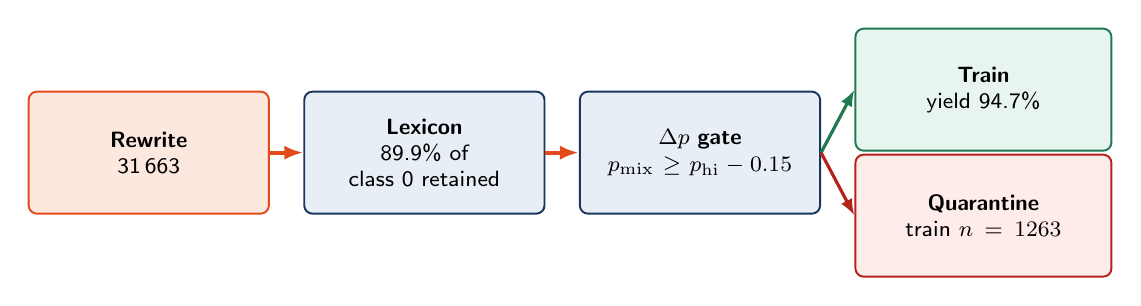
\begin{tikzpicture}
  \node[card=sorange,fill=orangesoft,text width=2.7cm] (r) at (0,0.9) {\textbf{Rewrite}\\31\,663};
  \node[card=snavy,fill=navysoft,text width=2.7cm] (lex) at (3.5,0.9) {\textbf{Lexicon}\\89.9\% of class~0 retained};
  \node[card=snavy,fill=navysoft,text width=2.7cm] (dp) at (7.0,0.9) {\textbf{$\Delta p$ gate}\\$p_{\mathrm{mix}}\ge p_{\mathrm{hi}}-0.15$};
  \draw[flowline] (r) -- (lex); \draw[flowline] (lex) -- (dp);
  \node[card=sok,fill=oksoft,text width=2.9cm] (ok) at (10.6,1.7) {\textbf{Train}\\yield 94.7\%};
  \node[card=sbad,fill=badsoft,text width=2.9cm] (bad) at (10.6,0.1) {\textbf{Quarantine}\\train $n=1263$};
  \draw[arr,sok] (dp.east) -- (ok.west);
  \draw[arr,sbad] (dp.east) -- (bad.west);
\end{tikzpicture}
\end{center}
\vspace{0.15em}
\term{quarantine}{Held-out rejected rewrites with a reason: score drop, missing lexicon stem, collapsed length, refusal, leftover Devanagari. Not deleted. Not in train.}
\end{frame}

% ------------------------------------------------------------------
\begin{frame}{Hinglish evaluation is frozen at $n=6368$ before training.}
\begin{center}
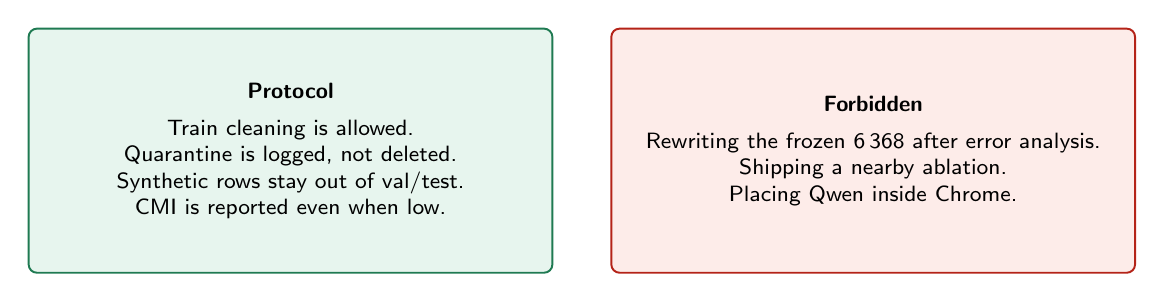
\begin{tikzpicture}
  \node[card=sok,fill=oksoft,text width=6.3cm,minimum height=3.1cm] at (0,0)
    {\textbf{Protocol}\\[4pt]Train cleaning is allowed.\\Quarantine is logged, not deleted.\\Synthetic rows stay out of val/test.\\CMI is reported even when low.};
  \node[card=sbad,fill=badsoft,text width=6.3cm,minimum height=3.1cm] at (7.4,0)
    {\textbf{Forbidden}\\[4pt]Rewriting the frozen 6\,368 after error analysis.\\Shipping a nearby ablation.\\Placing Qwen inside Chrome.};
\end{tikzpicture}
\end{center}
\vspace{0.4em}
{\footnotesize Moving the test after error analysis would make 84.36\% incomparable to the poster. Layer-1 cleaning and 977 synthetic rows were tried on train only.}
\end{frame}

% ------------------------------------------------------------------
\begin{frame}{Omitting Hindi MACD collapses Devanagari accuracy to 70.04\%.}
\begin{center}
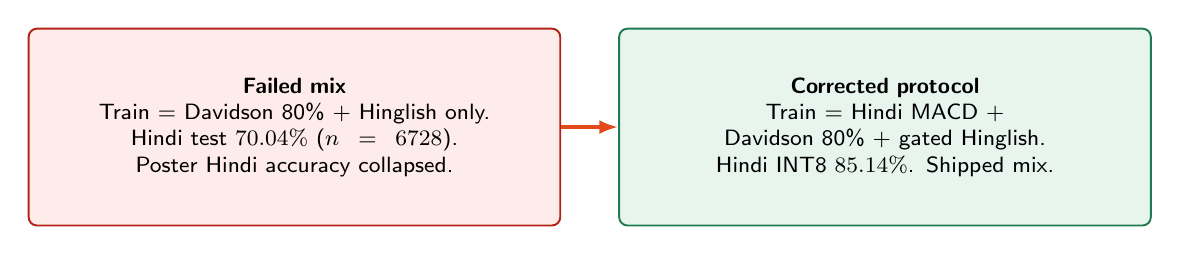
\begin{tikzpicture}
  \node[card=sbad,fill=badsoft,text width=6.4cm,minimum height=2.5cm] (fail) at (0,0.9)
    {\textbf{Failed mix}\\Train $=$ \mbox{Davidson} 80\% $+$ Hinglish only.\\Hindi test $70.04\%$ ($n=6728$).\\Poster Hindi accuracy collapsed.};
  \node[card=sok,fill=oksoft,text width=6.4cm,minimum height=2.5cm] (fix) at (7.5,0.9)
    {\textbf{Corrected protocol}\\Train $=$ Hindi MACD $+$ \mbox{Davidson} 80\% $+$ gated Hinglish.\\Hindi INT8 $85.14\%$. Shipped mix.};
  \draw[flowline] (fail) -- (fix);
\end{tikzpicture}
\end{center}
\vspace{0.25em}
{\footnotesize Corrected sizes: train 58\,929 / val 15\,581 / test 15\,575. A Hinglish gain that costs Hindi is not adopted.}
\end{frame}

% ------------------------------------------------------------------
\begin{frame}{Shipped INT8 Hinglish accuracy is 84.36\% with A--B--C unchanged.}
\begin{center}
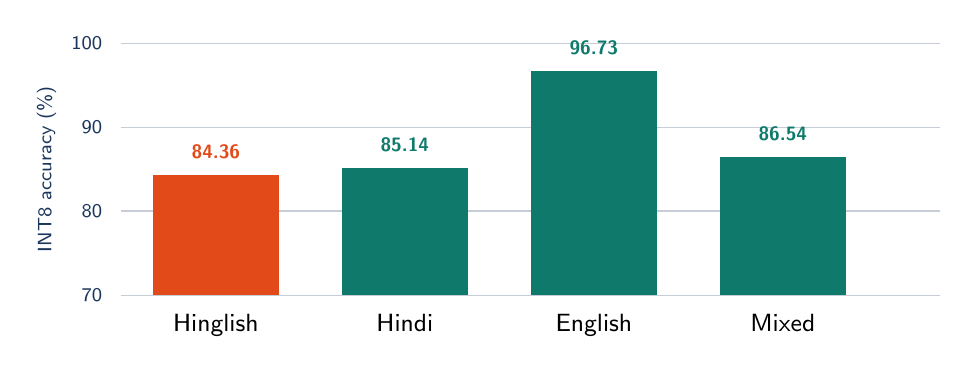
\begin{tikzpicture}
  \foreach \y/\lab in {0/70, 1.07/80, 2.13/90, 3.2/100} {
    \draw[snavy!25] (0,\y) -- (10.4,\y);
    \node[font=\scriptsize\sffamily,anchor=east,text=snavy] at (-0.12,\y) {\lab};
  }
  \fill[sorange] (0.4,0) rectangle (2.0,1.53);
  \node[font=\scriptsize\sffamily\bfseries,text=sorange] at (1.2,1.82) {84.36};
  \node[font=\small\sffamily,anchor=north] at (1.2,-0.12) {Hinglish};
  \fill[steal] (2.8,0) rectangle (4.4,1.62);
  \node[font=\scriptsize\sffamily\bfseries,text=steal] at (3.6,1.91) {85.14};
  \node[font=\small\sffamily,anchor=north] at (3.6,-0.12) {Hindi};
  \fill[steal] (5.2,0) rectangle (6.8,2.85);
  \node[font=\scriptsize\sffamily\bfseries,text=steal] at (6.0,3.14) {96.73};
  \node[font=\small\sffamily,anchor=north] at (6.0,-0.12) {English};
  \fill[steal] (7.6,0) rectangle (9.2,1.76);
  \node[font=\scriptsize\sffamily\bfseries,text=steal] at (8.4,2.05) {86.54};
  \node[font=\small\sffamily,anchor=north] at (8.4,-0.12) {Mixed};
  \node[rotate=90,font=\scriptsize\sffamily,text=snavy] at (-0.95,1.6) {INT8 accuracy (\%)};
\end{tikzpicture}
\end{center}
{\footnotesize Frozen Hinglish $n=6368$. Mixed 86.54\% is lower than poster 88.01\% because Hinglish is now inside the mix. Same MiniLM, 113\,MB, 28\,ms.}
\end{frame}

% ------------------------------------------------------------------
\begin{frame}{HinGE: Hindi-only Qwen versus WAC and PAC}
\begin{center}
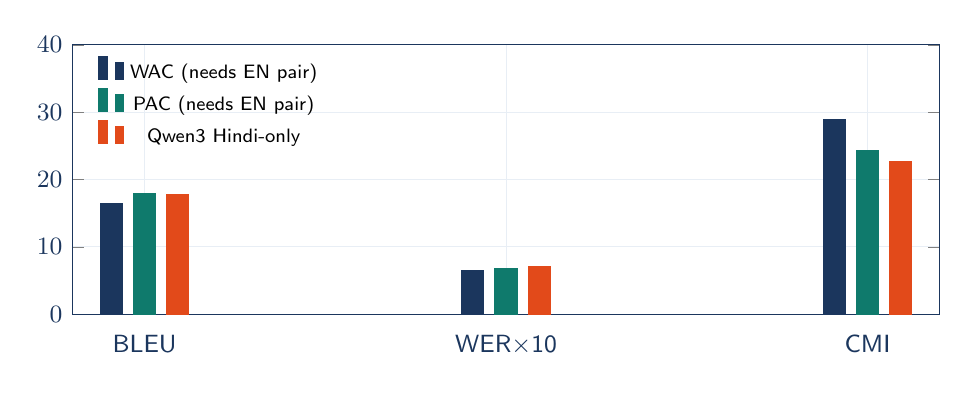
\begin{tikzpicture}
\begin{axis}[
  ybar=4pt, bar width=8pt,
  width=12.6cm, height=5.0cm,
  ymin=0, ymax=40,
  symbolic x coords={BLEU, WER$\times$10, CMI},
  xtick=data,
  legend style={font=\scriptsize\sffamily, at={(0.02,0.98)}, anchor=north west, draw=none, fill=none},
  axis line style={snavy},
  tick label style={font=\small\sffamily,color=snavy},
  grid=major, grid style={navysoft},
  xtick style={draw=none},
]
\addplot[fill=snavy,draw=snavy] coordinates {(BLEU,16.4) (WER$\times$10,6.5) (CMI,28.9)};
\addplot[fill=steal,draw=steal] coordinates {(BLEU,17.9) (WER$\times$10,6.7) (CMI,24.3)};
\addplot[fill=sorange,draw=sorange] coordinates {(BLEU,17.7) (WER$\times$10,7.1) (CMI,22.7)};
\legend{WAC (needs EN pair), PAC (needs EN pair), Qwen3 Hindi-only}
\end{axis}
\end{tikzpicture}
\end{center}
{\footnotesize Human HinGE CMI $=35.6$. This table evaluates the \emph{converter}. It does not replace detector accuracy.
\term{BLEU}{Precision against a human Hinglish reference. Not abuse-detection accuracy.}}
\end{frame}

% ------------------------------------------------------------------
\begin{frame}{MACD rewrites mix more shallowly than HinGE human references.}
\begin{columns}[T,onlytextwidth]
\begin{column}{0.46\textwidth}
\vspace{-0.4em}
\[
\mathrm{CMI}=100\left(1-\frac{\max_i w_i}{n}\right)
\]
{\scriptsize $n$: language-tagged tokens (no emojis). $w_i$: count in language $i$. CMI $=0$ if only one language remains.}
\end{column}
\begin{column}{0.52\textwidth}
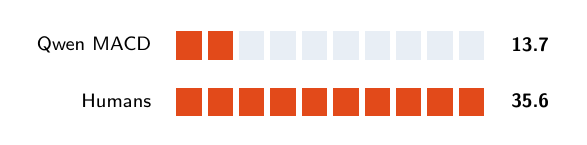
\begin{tikzpicture}[scale=0.95]
  \node[font=\scriptsize\sffamily,anchor=east] at (-0.2,1.1) {Qwen MACD};
  \node[font=\scriptsize\sffamily,anchor=east] at (-0.2,0.35) {Humans};
  \foreach \i in {0,1} {\fill[sorange] (\i*0.42,0.9) rectangle (\i*0.42+0.34,1.28);}
  \foreach \i in {2,...,9} {\fill[navysoft] (\i*0.42,0.9) rectangle (\i*0.42+0.34,1.28);}
  \foreach \i in {0,...,9} {\fill[sorange] (\i*0.42,0.15) rectangle (\i*0.42+0.34,0.53);}
  \node[font=\scriptsize\sffamily\bfseries,anchor=west] at (4.35,1.1) {13.7};
  \node[font=\scriptsize\sffamily\bfseries,anchor=west] at (4.35,0.35) {35.6};
\end{tikzpicture}\\[0.4em]
{\scriptsize 25\% of Qwen MACD lines have CMI $=0$ (romanized Hindi or English, not a mix).}
\end{column}
\end{columns}
\end{frame}

% ------------------------------------------------------------------
\begin{frame}{Layer-1 and synthetic rows do not improve the freeze.}
\begin{center}
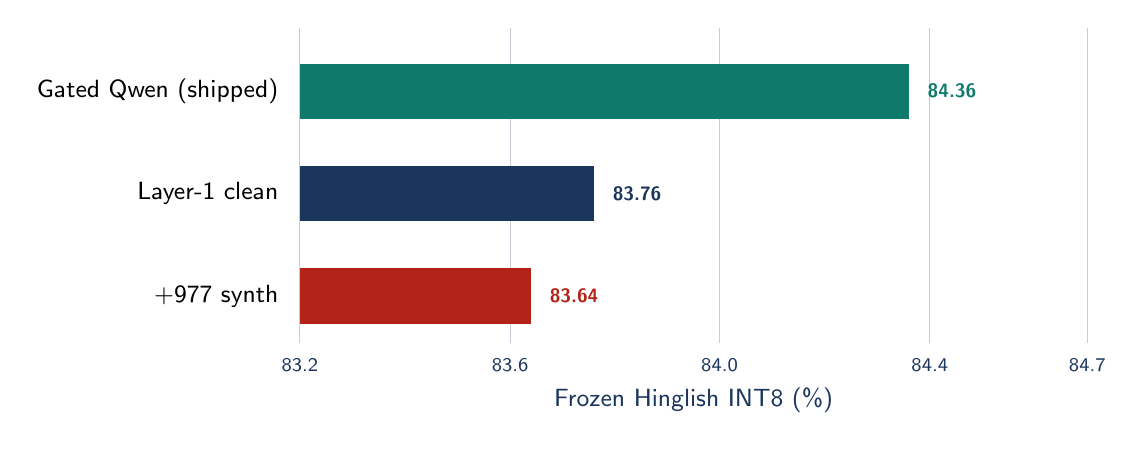
\begin{tikzpicture}
  \foreach \x/\lab in {0/83.2, 2.67/83.6, 5.33/84.0, 8.0/84.4, 10.0/84.7} {
    \draw[snavy!25] (\x,0) -- (\x,4.0);
    \node[font=\scriptsize\sffamily,anchor=north,text=snavy] at (\x,-0.08) {\lab};
  }
  % map v -> (v-83.2)/1.5 * 10
  \fill[steal] (0,2.85) rectangle (7.73,3.55);
  \node[font=\small\sffamily,anchor=east] at (-0.15,3.20) {Gated Qwen (shipped)};
  \node[font=\scriptsize\sffamily\bfseries,text=steal,anchor=west] at (7.85,3.20) {84.36};
  \fill[snavy] (0,1.55) rectangle (3.73,2.25);
  \node[font=\small\sffamily,anchor=east] at (-0.15,1.90) {Layer-1 clean};
  \node[font=\scriptsize\sffamily\bfseries,text=snavy,anchor=west] at (3.85,1.90) {83.76};
  \fill[sbad] (0,0.25) rectangle (2.93,0.95);
  \node[font=\small\sffamily,anchor=east] at (-0.15,0.60) {+977 synth};
  \node[font=\scriptsize\sffamily\bfseries,text=sbad,anchor=west] at (3.05,0.60) {83.64};
  \node[font=\small\sffamily,text=snavy] at (5.0,-0.72) {Frozen Hinglish INT8 (\%)};
\end{tikzpicture}
\end{center}
\vspace{0.1em}
{\footnotesize\parbox{\linewidth}{Deltas $-0.60$ and $-0.72$ on the same freeze. Synthetic rows never entered test. The nearby recipes are not shipped.}}
\end{frame}

% ------------------------------------------------------------------
\begin{frame}{Largest validation errors are noisy MACD gold, not obfuscation.}
\begin{center}
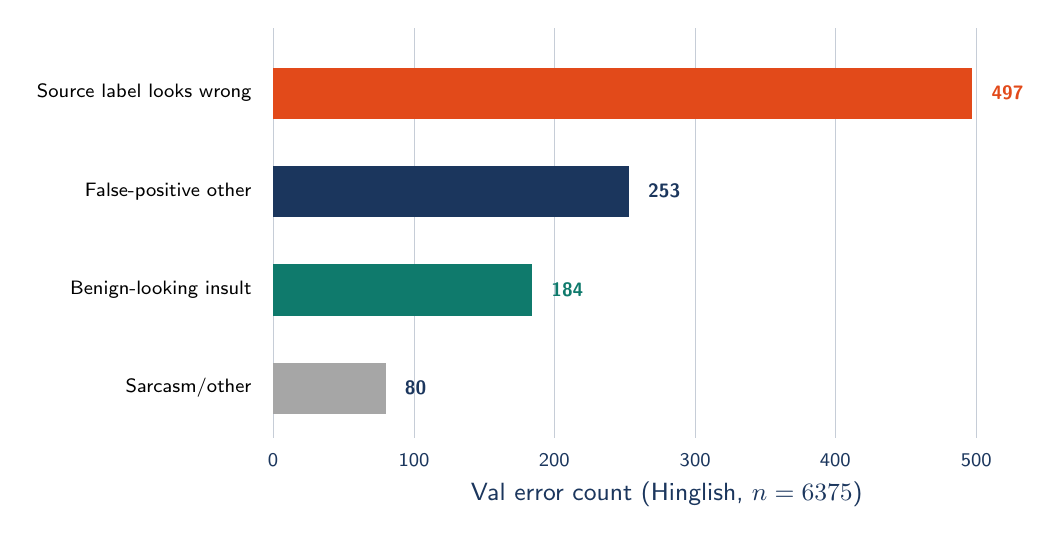
\begin{tikzpicture}
  \foreach \x/\lab in {0/0, 1.79/100, 3.57/200, 5.36/300, 7.14/400, 8.93/500} {
    \draw[snavy!25] (\x,0) -- (\x,5.2);
    \node[font=\scriptsize\sffamily,anchor=north,text=snavy] at (\x,-0.08) {\lab};
  }
  % map count -> count/560 * 10
  \fill[sorange] (0,4.05) rectangle (8.88,4.70);
  \node[font=\scriptsize\sffamily,anchor=east] at (-0.15,4.38) {Source label looks wrong};
  \node[font=\scriptsize\sffamily\bfseries,text=sorange,anchor=west] at (9.00,4.38) {497};
  \fill[snavy] (0,2.80) rectangle (4.52,3.45);
  \node[font=\scriptsize\sffamily,anchor=east] at (-0.15,3.13) {False-positive other};
  \node[font=\scriptsize\sffamily\bfseries,text=snavy,anchor=west] at (4.64,3.13) {253};
  \fill[steal] (0,1.55) rectangle (3.29,2.20);
  \node[font=\scriptsize\sffamily,anchor=east] at (-0.15,1.88) {Benign-looking insult};
  \node[font=\scriptsize\sffamily\bfseries,text=steal,anchor=west] at (3.41,1.88) {184};
  \fill[black!35] (0,0.30) rectangle (1.43,0.95);
  \node[font=\scriptsize\sffamily,anchor=east] at (-0.15,0.63) {Sarcasm/other};
  \node[font=\scriptsize\sffamily\bfseries,text=snavy,anchor=west] at (1.55,0.63) {80};
  \node[font=\small\sffamily,text=snavy] at (5.0,-0.72) {Val error count (Hinglish, $n=6375$)};
\end{tikzpicture}
\end{center}
\vspace{0.1em}
{\footnotesize\parbox{\linewidth}{507 false positives, 528 missed abuse. Cluster labels are a research reading, not a second gold. Cleaning this on the \emph{test} set is exactly what the freeze forbids.}}
\end{frame}

% ------------------------------------------------------------------
\begin{frame}{Closed results and remaining measurement}
\begin{center}
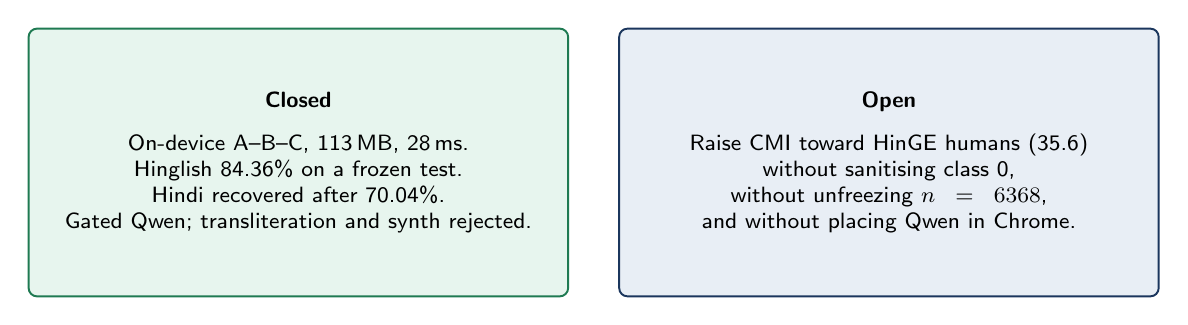
\begin{tikzpicture}
  \node[card=sok,fill=oksoft,text width=6.5cm,minimum height=3.4cm] at (0,0)
    {\textbf{Closed}\\[6pt]On-device A--B--C, 113\,MB, 28\,ms.\\Hinglish 84.36\% on a frozen test.\\Hindi recovered after 70.04\%.\\Gated Qwen; transliteration and synth rejected.};
  \node[card=snavy,fill=navysoft,text width=6.5cm,minimum height=3.4cm] at (7.5,0)
    {\textbf{Open}\\[6pt]Raise CMI toward HinGE humans (35.6)\\without sanitising class 0,\\without unfreezing $n=6368$,\\and without placing Qwen in Chrome.};
\end{tikzpicture}
\end{center}
\end{frame}

\end{document}
